\documentclass[12pt,a4paper]{article}
\usepackage[a4paper]{geometry}
\usepackage{array}
\usepackage{hhline}
\usepackage{graphics}
\usepackage{csvsimple}
\usepackage[russian,english]{babel}
\usepackage[utf8]{inputenc}
\usepackage[T2A]{fontenc} 
\usepackage{ulem}
\usepackage{cmap}
\usepackage{makecell}
\usepackage{ifpdf}
\setlength\extrarowheight{2pt}
\setlength{\parindent}{0cm}
\newcommand{\phylentry}[6] {\\\hline\makecell{
#1\medskip\\
\hhline{|-|}
\\#2\\#3\medskip\\
\hhline{|-|}\\
{#6}}
&\makecell{#4}&\makecell{#5}}
%Syntax: \phylentry{Who}{When}{Where}{Phylosophy}{NotPhylosophy}{ETC} // currently ETC is not used
\hoffset -1.6cm 
\textwidth  16.5cm 
\textheight 24cm 
%\topmargin -1cm 
\parskip 8pt 
\setlength{\unitlength}{1cm}
\sloppy
\addto\captionsenglish{
\renewcommand{\contentsname}{{\bf CO}ntents}
\renewcommand{\refname}{Bibliography}
\renewcommand{\figurename}{Figure}
\renewcommand{\tablename}{Table}
\renewcommand{\abstractname}{Abstract}
\renewcommand{\partname}{Section}
\renewcommand{\bottomfraction}{0.5}
\renewcommand{\floatpagefraction}{0.4}
\renewcommand{\textfloatsep}{0.5cm}
\renewcommand{\intextsep}{0.6cm}
\renewcommand{\floatsep}{0.3cm}
}

\renewcommand\theadalign{cb}
\renewcommand\theadfont{\bfseries}
\renewcommand\theadgape{\Gape[4pt]}
\renewcommand\cellgape{\Gape[4pt]}
%<pics>
\newcommand{\materialist}[0]{\includegraphics{dummy-achievement.png}}%</pics>
\begin{document}
%..................................................................
\begin{titlepage}
\par 
\vspace*{-2cm}
\begin{center}
{\sf \Large
\vspace*{1.5cm}
{\Huge Семенов, 9-й семестр, 2017}\\
{ Философия, эпизод 2:}\\
{ Больше конспектов \sout{Богу} Абсолютному духу конспектов}}\\

\vspace*{2cm}
\scalebox{1.2}{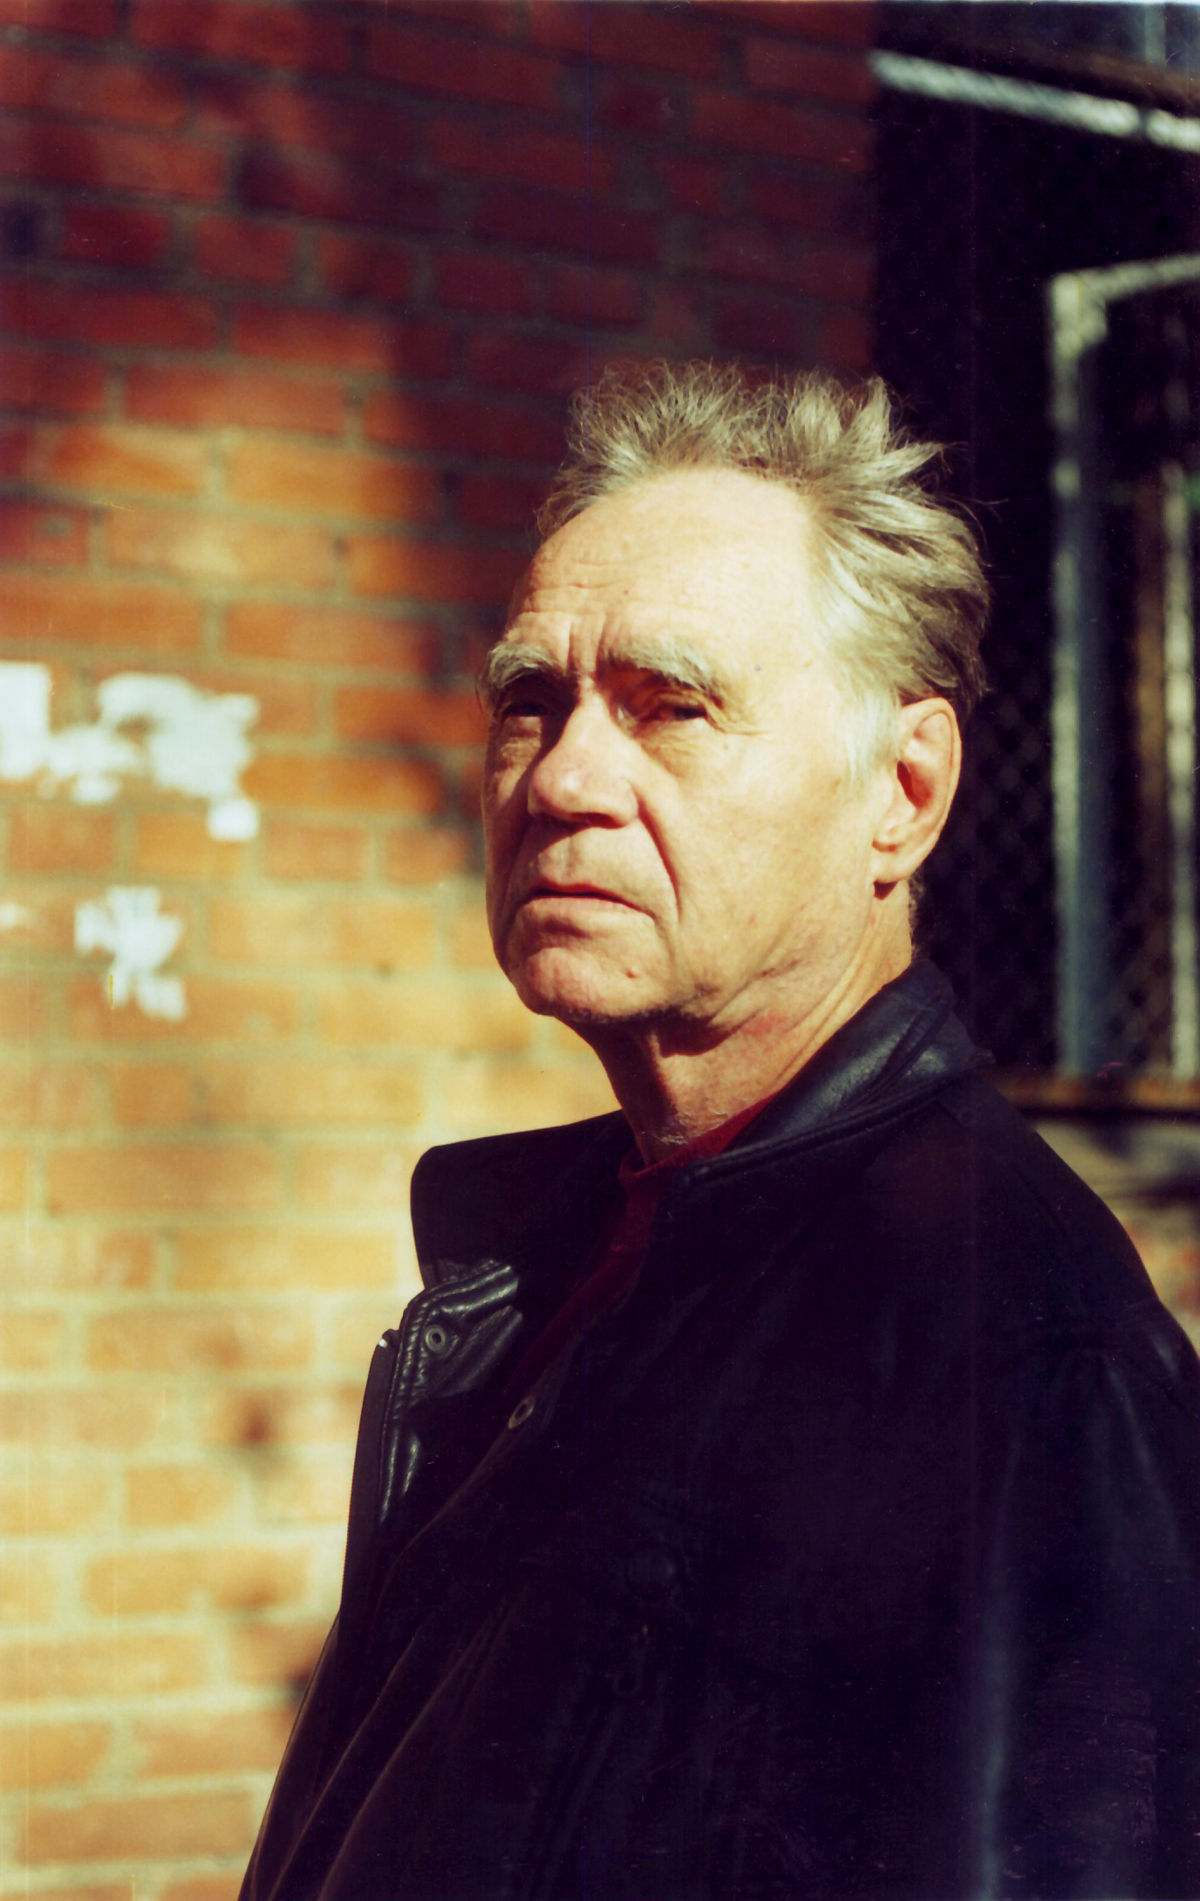
\includegraphics{thegod.jpg}} \\
{\small }
\begin{flushright}
\sl\small
by Nyaxx11k aka KingKO
\end{flushright}
\end{center}
\end{titlepage}
%..................................................................
\topmargin -1cm 
\hoffset -0.7in 
\textwidth 6.0in 
\textheight 9.0in 
\normalsize 
\pagenumbering{arabic}
%----------------
\tableofcontents
\pagebreak
%----------------

\section{Философия как наука об истине, теория познания и самый общий метод исследования}
\textit{Этот вопрос будет длинный... Итак, есть несколько взглядов на философию. Семенов придерживается того, что философия - это все же наука. Да, покукарекать за жизнь на кухне - НЕ философия.} \textbf{Философия} - это наука об истине. Конечно, это не значит, что остальные науки о заблуждении. Все науки ищут истину. Философия наука об истине именно в том смысле, что ищет истину о самой истине. Т.е. как мыслить правильно, чтобы достичь истины и не скатиться в \sout{РЕН-ТВ} заблуждение. То есть, философия есть теория познания (ака \textbf{гносеология}/\textbf{эпистемология}. Вроде, под ними многие понимают немного разные вещи, но для нас это синонимы). Ясно, что для этого философия должна разработать общий метод мышления, т.е. философия еще и наука и о наиболее общем методе познания. При этом она сама и есть этот общий метод мышления, а также и наиболее общий метод мышления. \textit{Ах да, \textbf{истина} - это то, что согласуется с действительностью, соответствие между миром и сознанием. В билетах этого не видно, но помнить будет не лишним}. 

\section{Основной вопрос философии}
"Что первично - \textbf{мир} или \textbf{сознание}?". Ну а теперь разберемся, почему же он основной. Нам необходимо дать определение мира и сознание. Обычно мы даем их через род и видовое отличие: например, студент - учащийся высшего учебного заведения. "Учащийся" - род, "высшего учебного заведения" - видовое отличие. И эта схема прекрасно работает, пока мы не дойдем до предельно общих понятий: мира и сознания, которые разделяют второе место по обощенности. На первом, конечно же, \textbf{бытие}, т.е. все. Вообще все. Соответственно, сказать, что и мир, и сознание - бытие - это ничего не сказать. Значит, определить их можно, только раскрыв их отношение: что из них первично, а что вторично. \textit{Собственно, с помощью этого вопроса классифицируют сорта философов. Главных направлений 2: \textbf{материализм} и \textbf{идеализм}. Есть еще побочные направления, у которых первично что-то третье/первичны две и более вещей/вообще неизвестно, что первично, и никогда не будет известно. Все они, правда в той или иной мере тяготеют к идеализму. Семенов даже говорил, что есть материалисты и все остальные.}

\section{Философия как мировоззрение (онтология). Натурфилософия. Философия истории.}
Итак, мы выяснили, что философия - наука об истине, а ее основной вопрос - "Что первично - мир или сознание?". Но это означает, что философия дает предельно общее мировоззрение и предельно общий взгляд на бытие. Т.е. философия - \textbf{онтология}. Раньше философия еще давала предельно общую картину мира - другие науки еще были в зачаточном состоянии, и только философия была готова дать хоть что-то. Такое учение называется \textbf{натурфилософией}. В настоящее время натурфилософия отмерла за ненадобностью. \textit{Но не онтология - она по прежнему занимается проблемами мира - теми, которые нужны для теории познания}. Но кроме природы есть еще общество - им занимаются \textbf{социальная философия} и \textbf{философия истории}. И с ними все не так однозначно, как с натурфилософией. Во-первых, есть \textbf{общественное сознание} - в широком смысле это все знание человечества; более того, сознание отдельного человека формируется в обществе \textit{(а дети-Маугли ни говорить, ни социализироваться не могут)}. Во-вторых, разные школы придерживаются разных взглядов на общество: первые говорят, что общество - только название, а на самом деле есть только взаимодействующие люди. Вторые таки признают общество. Это два направления - \textbf{социальный номинализм} и \textbf{социальный реализм} соответственно.

\section{Научная революция XVII века}
\textit{Ну, с общими вопросами разобрались, теперь поехали по философам.} Итак, наука окончательно сформирофалась в 17 в. \textit{Вообще, знание было всегда, но раньше оно было бессистемным и бездоказательным. В Древнем Египте, например, умели решать квадратные уравнения, но рецепт был получен методом тыка. Первое доказательство появилось только в 6 в. д.н.э. (привет, Фалес Милетский). Тогда, правда, наука смешивалась с натурфилософией аки нейтрино. С вытекающими отсюда переходами одного в другое. Окончательно же труЪ-наука сформировалась в 17 в.}
Ну и пробежимся по ученым того времени (спискота):

\underline{Леонардо да Винчи (1452-1519)}. Художник, изобретатель. Человек у него лишь первый из зверей, а душа не бессмертна. Один из первых \textbf{эмпириков} - ценил опыт, но и чистый эмпиризм без анализа отвергал. Развивал математику.

\underline{Николай Коперник (1473-1543)}. В книге "Об обращении небесных сфер" ввел математически обоснованную гелиоцентрическую систему. Утверждал, что это лишь способ уточнить расчеты (правда, его модель была далеко не идеальна). Говорил, что это гипотетически, боялся публиковаться. Еще бы - Церкви это ой как не понравилось. Правда, Церковь тогда была занята реформацией, а потом работа разошлась, а Коперник в тот же год благоразумно умер, и все: поздняк метяться, Земля - не центр мироздания, Бог не может жить на небесной тверди по прицине отсутствия оной. Пришлось закинуть Бога за орбиту Сатурна (то, что есть еще Уран и Нептун, никто не догадывался).

\underline{Джордано Бруно (1548-1600)}. Философ, естествоиспытатель. В работах жег не по-детски. Мир бесконечен, звезды - те же солнца, с планетами и разумной жизнью. Инопланетян что, тоже Христос создал? Вот и получается, что Бога нет. Да, в Средневековье была популярна концепция двух истин - разума и откровения. Так вот, нет двух истин - есть только истина разума, а религия - бред собачий.  Правда, мировая душа у него все-таки была, но это нечто глобальное и пассивное. У церкви с такого пригорело, однако в 1600 году на Площади Цветов во Флоренции она взяла реванш. Особый цинизм ситуации заключался в том, что костер считался гуманной казнью, так как не приводил к пролитию крови. \textit{Однако, эпопея с горящими пердаками продолжается. Так, недавно поставили Джордано на этой самой Площади Цветов памятник - дескать, мученник науки, сгорел на работе, можно сказать (\textit{Вечный огонь поставьте}). Так вот, верующие раскукарекались. А узнай Джордано, что в 21 веке в одной стране поп кандидатскую по теологии защитил - сгорел бы и без дров.}

\underline{Галилео Галилей(1564-1642)}. Астроном, создатель первого телескопа (правда, подзорная труба була уже до него). Изучил Луну. Открыл спутники Юпитера (4 самых крупных). Еще и механик - опроверг положение Аристотеля о разной скорости падения тел. Изучал динамику пушечного ядра - даже в баллистики приглашали. Ну и маятник. Написал "Диалог о двух системах мира" (Птолемей vs Коперник - защищает Коперника). Написал на итальянском, а не на латыни. Слетелись инквизиторы и заставили публично отречься. Галилей отрекся (есть легенда, что в конце он произнес "И все-таки она вертится". Пруфов нет).  

\underline{Иоганн Кеплер (1571-1646)}. Опять астроном, открыл три закона обращения планет (\textit{вспомним общефиз, 1-й семестр?})

\underline{Уильям Гильберт (1540-1603)}. \textit{Не путать с Давидом Гильбертом - тот из 20-го века.} Наука и до Англии добралась. Изучал магнит, открыл джва его полюса, понял, что у Земли тоже есть магнитное поле. Еще изучал электростатику, открыл, что не только янтарь электризуется.

\underline{Уильям Горвей (1578-1657)}. Открыл кровооброщение. Основоположник физиологии и эмбриологии.

\underline{Эванжелиста Торричелли (1608-1646)}. Открыл атмосферное давление и изобрел ртутный барометр. Создал гидродинамику.

\underline{Отто фон Герике (1602-1686)}. Открыл атмосферное давление и изобрел ртутный барометр. Создал гидродинамику.

\underline{Роберт Бойль (1627-1691)}. Открыл закон имени себя-Мариотта. Создал научную химию.

\underline{Эдм Мариотт (1620-1684)}. Открыл закон имени Бойля-себя. Создал французскую академию наук.

\underline{Христиан Гюйгенс (1629-1691)}. Открыл кольца Сатурна, создал маятниковые и пружинно-балансирные часы. Моряки сказали спасибо, ибо без них долготу корабля фиг определишь. Создал теорию маятника и волновую теорию света.

\underline{Антон ван Левенгук (1632-1723)}. Изобрел микроскоп. Открыл бактерии, изапилил микробиологию. \textit{А однажды плюнул под микроскоп. Посмотрев на зоопарк полости рта, стал чистить зубы еще до того, как это стало мейнстримом.}

\underline{Роберт Гук (1635-1705)}. Закон имени себя.

\underline{Исаак Ньютон (1642-1716)}. 3 закона имени себя + закон всемирного тяготения + матан, независимо от Лейбница. Сделал механику точной наукой. Топил за корпускулярную теорию света - \textit{создатель квантмеха (нет)}
 
На этом спискота все. Итого 12 ученых. А если в общем - ученые стали ставить эксперименты (систематические), юзать приборы - всякие теле-микро-скопы, баро-термометры, часы. Появились обсерватории. В Англии Карл II запилил первую академию наук - т.н. "Королевское общество" (1662). Потом тренд подхватили Франция, Пруссия, а там и в Россию завезли. Ученые стали делать доклады, а сборники этих докладов стали первой научной прессой. Потом, когда ученых стало побольше, уже и нормальная периодика пошла. Появилось и научное мышление. Чудеса наука не рассматривала. Да, гнать на церковь по-прежнему было накладно, но это уже шаг вперед . Появилась концепция \textbf{детерминизма} - учения о всеобщей причинности и предопределенности событий. Потом и теорвер появился. Он с детерминизмом прекрасно уживался - все случайности проистекают из нашего недостаточного знания, а на самом деле все предопрелелено. Тут нужно упомянуть Лапласа с его демоном. Если демон знает коориднаты и скорости всех тел, а также имеет бесконечную разрядность и производительность, он сможет просчитать все события в нашем мире. Такой вот \textbf{механистический детерминизм}. \textit{Правда, квантовая механика похоронила абсолютный детерминизм, но в пропатченных вариантах он жив}.
%Smth else?

\section{Западноевропейская классическая философия XVII - первой половины XIX вв. Эмпиризм и рационализм.}
Итак, окончательно сформировалась наука. И тем самым у философов появилась пища для ума. Откуда берется научное знание? Как мыслить так, чтобы полученные теории действительно работали? \textit{Тут нужно сказать, что есть два вида знания - \textbf{житейское} и \textbf{научное}. Первое - бессистемное и бездоказательное, полученное в ходе повседневной человеческой деятельности. Второе же и системное, и обосновывается. Например, счет на пальцах у древних людей - это житейское знание. А аксиоматика Пеано - научное}. Надо сказать, еще Бэкон (который Роджер) выделял три источника знания - авторитет, ум и опыт. То, что авторитет может ошибаться - и так понятно. А с умом и опытом сложнее. И тут возникли два направления - \textbf{эмпиризм} и \textbf{рационализм}.

Эмпиристы утверждают, что единственный источник знания - опыт (Р. Бэкон, к слову, тоже придерживался этой мысли). \textbf{Априорного}, т.е.полученного без опыта знания у них нет - только  \textbf{апостериорное}. Да, самое главное: а что есть \textbf{опыт}? Ну, опыт бывает житейский и научный. С ними все примерно так же, как и со знанием. Житейский получается в ходе человеческой практики - хочешь, чтобы что-то заработало - делай так-то, а так-то, наоборот, не делай. Научный - продуманный, системный, знание, полученное в ходе него, фиксируется в суждениях, т.е. становится \textbf{фактом}. Нельзя сказать, что все эмпирики отвергают разум: многим он нужен для обработки экспериментальных данных в теории. Т.е. сначала эмпирический уровень знания, а потом и теоретический. Есть же и \textbf{сенсуалисты} - у них в разуме нет ничего, чего не было бы в чувствах (\textit{ага, многие из вас видели отдельные атомы?}).

Рационалисты, напротив, говорили, что априорное знание есть, и более того, оно даже круче апостериорного: опыт может раз сработать, два сработать, а на третий раз слажать, а вот что доказано умом - то работает всегда.

А где же истина? А она, как всегда, где-то рядом. Действительно, мир дан нам только в наших чувствах - правы сенсуалисты. Но разум в состоянии раскрывать закономерности, находить причинно-следственные связи и создавать реально работающие (разумеется, с определенной точностью и в определенных границах) теории - правы рационалисты. Так что, все эти направления - это, как правило, раздувание одной стороны истины в ущерб другим.

\section{Философия Френсиса Бэкона}

\section{Философия Рене Декарта}
\section{Философия Томаса Гоббса}
\section{Философия Баруха Спинозы}
\section{Философия Готфрида Лейбница}
\section{Философия Джона Локка}
\section{Учение Джона Локка о первичных и вторичных качествах}
\section{Философия Джорджа Беркли}
\section{Философия Давида Юма. Обоснование им феноменализма (агностицизма).}
\section{Основные идеи века Просвещения}
\section{Возникновение первых научных периодизаций мировой истории и концепции прогресса (человеческого общества Адам Фергюсон, Адам Смит, Жак Тюрго, Жан Кондорсе).}
\section{Жан-Жак Руссо, Морелли, Габриэль де Мабли}
\section{Географический детерминизм. Ш. Монтескье.}
\section{Демографический детерминизм.  К.А. Гельвеций и А. Барнав.}
\section{Вольтер}
\section{Жан Мелье}
\section{Борьба французских материалистов XVIII в. против идеализма и религии}
\section{Учение французских материалистов XVIII в. о природе. Их механицизм и абсолютный детерминизм}
\section{Теория познании французских материалистов}
\section{Учение французских материалистов XVIII в.  об обществе и истории}
\section{Немецкая классическая философия}
\section{Иммануил Кант.  Жизнь и развитие его философской мысли.}
\section{Учение Иммануила Канта о ноуменах (вещах в себе) и феноменах (вещах для нас)}
\section{Априоризм Иммануила Канта}
\section{Иммануил Кант о синтезе чувственности и рассудка}
\section{Открытия Иммануила Канта. Рациональное зерно, содержащееся в его гносеологической концепции.}
\section{Иммануил Канта о разуме. Антиномии разума.}
\section{Жизнь и философия Иоганна Готлиба Фихте}
\section{Жизнь и философия Фридриха Вильгельма Йозефа Шеллинга}
\section{Георг Вильгельм Фридрих Гегель. Его жизнь и основные работы.}
\section{Проблема истины в "Феноменологии духа" Георга Гегеля}
\section{Открытие Георгом Гегелем мышления как объективного процесса. Гегелевская диалектика.}
\section{Философская система Георга Гегеля}
\section{Наука логики Георга Гегеля}
\section{Философия природы Георга Гегеля}
\section{Философия духа Георга Гегеля}
\section{Противоречие между методом и системой в философии Георга Гегеля}
\section{Великая Французская революция и крах волюнтаризма.  Философия истории Георга Гегеля. }
\section{Раскол в школе Г. Гегеля. Младогегельянцы (Давид Штраус, Бруно Бауэр).}
\section{Антропологический материализм Людвига Фейербаха}
\section{Кризис материализма на рубеже XVIII–XIX вв.}
\section{Исторические предпосылки возникновение марксизма. Основные части марксизма.}
\section{К. Маркс и Ф. Энгельс как создатели марксизма. Эволюция их взглядов.}
\section{Философская и обществоведческая мысль в поисках объективного источника общественных идей. Французские историки эпохи Реставрации.}
\section{Философская и обществоведческая мысль в поисках объективного источника общественных идей. Открытие экономических отношений и возникновение политический экономии.}
\section{Философская и обществоведческая мысль в поисках объективного источника общественных идей. Выделение основных эпох истории цивилизованного общества.}
\section{Философия истории А. Сен-Симона.}
\section{Экономический детерминизм Ричарда Джонса.}
\section{Создание материалистического понимания истории и его основные понятия.}
\section{Возникновение диалектического материализма и его отличие от всех предшествующих материалистических систем.}
\section{Возникновение диалектического материализма и его отличие от предшествующих материалистических систем}
\section{Классическая и неклассическая западноевропейская философии Нового времени. Их отличие и особенности их развития.}
\section{Основные течения западноевропейской постклассической философии: иррационализм, первый, второй и третий позитивизм, постпозитивизм, постмодернизм}

\end{document}
